\documentclass[10pt]{article} % Changed to article document class
\usepackage{tikz}
\usepackage{graphicx} % Added graphicx package for figures
\usepackage{amsmath} % Added for align environment for equations
\usepackage{cancel} % Added for the \cancel command

% Add title and author information
\title{Fourier Series \& Transformation} % Escaped ampersand in title
\author{Kirkwood Donavin -- Data Scientist} % Added addendum to author name
\date{} % Suppress date

\begin{document}

% Display the title and author
\maketitle

This document is a primer on the Fourier Series and how it is used to transform complex periodic functions into a useful Fourier approximation. These notes are for personal use but may be useful to others as well.

\section*{The Fourier Series} % Added a section title for context

A Fourier series is a way to represent a \textit{periodic} (e.g., seasonal) function as a sum of \textit{weighted} sine and cosine waves. They were first used by Joseph Fourier to find solutions to periodic functions that are not so easily differentiated as a series of sine and cosine functions. A fourier series looks like this:

\begin{align}
f(t) = a_0 & + a_1\cos(t) + a_2\cos(2t) + a_3\cos(3t) + ... \\
           & + b_1\sin(t) + b_2\sin(2t) + b_3\sin(3t) + ... \notag
\end{align}

Where $t$ is time. Note that the frequency for each added sine/cosine term is increasing.

\section*{Theory}

\subsection*{Derivation of Trigonometric Identies}

First, let us establish some trigonometric integration identities regarding these wave functions.

\begin{align}
    \int_0^{2\pi} \sin(mt)\mathrm{d}t &= 0 \\
    \intertext{\hspace{0.5cm} for \textit{any} integer $m$}
    \int_0^{2\pi} \cos(mt)\mathrm{d}t &= 0 \\
    \intertext{\hspace{0.5cm} for non-zero integer $m$}
    \int_0^{2\pi} \sin(mt) \cdot \cos(nt)\mathrm{d}t &= 0 \\
    \intertext{\hspace{0.5cm} for \textit{any} integers $m, n$}
    \int_0^{2\pi} \sin(mt) \cdot \sin(nt) &= 0 \\
    \intertext{\hspace{0.5cm} for integers $m,n$ when $m \neq n$ or $m \neq -n$}
    \int_0^{2\pi} \sin^2(mt)\mathrm{d}t &= \pi \\
    \intertext{\hspace{0.5cm} for integer $m = n \neq 0$, note this is the edge case of $m=n$ above}
    \int_0^{2\pi} \cos(mt) \cdot \cos(nt) &= 0 \\
    \intertext{\hspace{0.5cm} for integers $m,n$ when $m \neq n$ or $m \neq -n$}
    \int_0^{2\pi} \cos^2(mt)\mathrm{d}t &= \pi \\
    \intertext{\hspace{0.5cm} for integer $m = n \neq 0$} \notag
\end{align}

These are well known integral values, but I could use the integration review, so let us prove it. First, I will note the derivitive value of sine \& cosine:

\begin{align*}
    \frac{\mathrm{d}}{\mathrm{d}t}[\cos(mt)] & = m\cdot\left(-\sin(mt)\right) \\
    & = -m\sin(mt)\\
    &\text{And,}\\
    \frac{\mathrm{d}}{\mathrm{d}t}[\sin(mt)] & = m\cdot\left(\cos(mt)\right)
\end{align*}

The following is the integration of sine function for an arbitrary number $m$ of full periods.

\begin{align*}
    \int_0^{2\pi} \sin(mt)\mathrm{d}t & = -\frac1m\int_0^{2\pi}-m\sin(mt)\mathrm{d}t \\
    & = -\frac1m\left(\cos(mt)\right)\bigg\rvert_0^{2\pi} \\
    & = -\frac1m\left(\cancel{\cos(m\cdot2\pi)} - \cancel{\cos(m\cdot 0)}\right) \\
    & = -\frac1m\left(1 - 1\right) \\
    & = 0
\end{align*}

And, the integration of the cosine function for an arbitrary number $m$ of full periods:

\begin{align*}
    \int_0^{2\pi} \cos(mt)\mathrm{d}t & = \frac1m\int_0^{2\pi}m\cos(mt)\mathrm{d}t \\
    & = \frac1m\left(\sin(mt)\right)\bigg\rvert_0^{2\pi} \\
    & = \frac1m\left(\cancel{\sin(m\cdot2\pi)} - \cancel{\sin(m\cdot 0)}\right) \\
    & = -\frac1m\left(0 - 0\right) \\
    & = 0
\end{align*}

And, the integration of sine times cosine:

\begin{align*}
    \int_0^{2\pi}\sin(mt)\cos(nt)\mathrm{d}t & = \int_0^{2\pi}\frac12[\sin((m+n)t) +\sin((m-n)t)]\mathrm{d}t &\text{\hspace{0.5cm} by trigonometric identity} \\
    & = \frac12 \int_0^{2\pi}\sin((m+n)t)\mathrm{d}t + \frac12 \int_0^{2\pi}\sin((m-n)t)\mathrm{d}t\\
    & = \frac12 \cancel{\int_0^{2\pi}\sin(k\cdot t)\mathrm{d}t} + \frac12 \cancel{\int_0^{2\pi}\sin(l\cdot t)\mathrm{d}t} &\text{\hspace{0.5cm}  where $k=m+n$, and $l=m-n$ are integers}\\
    & = 0 &\text{By the integral identity of $\sin(mt)$ established above}
\end{align*}

And, the integration of sine times sine of different number of periods:

\begin{align*}
    \int_0^{2\pi} \sin(mt) \cdot \sin(nt) \mathrm{d}t &= \int_0^{2\pi}\frac12[\cos((m-n)t) - \cos((m+n)t) \mathrm{d}t \text{\hspace{0.5cm}by trigonometric identity, for $m \neq n, -n$.}&\\
    & =\frac12\cancel{\int_0^{2\pi}\cos((m-n)t)\mathrm{d}t} - \frac12\cancel{\int_0^{2\pi}\cos((m+n)t)\mathrm{d}t}\\
    & \text{Note that integer $k = m-n$ and $l = m+n$. Thus, for all integers $m \neq n, -n$:} &\\
    & = 0 \\
    & \text{However, if $m = n$, then we have:}\\
    \int_0^{2\pi} \sin^2(mt)\mathrm{d}t & = \frac12\int_0^{2\pi}\cos((\cancel{m-m})t)\mathrm{d}t - \frac12\cancel{\int_0^{2\pi}\cos((m+m)t)\mathrm{d}t}\\
    & = \frac12\int_0^{2\pi}1\mathrm{d}t\\
    & = \frac12 \cdot t \bigg\rvert_0^{2\pi} \\
    & = \frac12 (2\pi - 0) \\
    & = \pi
\end{align*}

And, the integration of cosine times cosine of different number of periods (nearly identical math to above):

\begin{align*}
    \int_0^{2\pi} \cos(mt) \cdot \cos(nt) \mathrm{d}t &=\int_0^{2\pi}\frac12[\cos((m-n)t) - \cos((m+n)t) \mathrm{d}t \text{\hspace{0.5cm}by trigonometric identity, for integers $m \neq n, -n$.}&\\
    & =\frac12\cancel{\int_0^{2\pi}\cos((m-n)t)\mathrm{d}t} - \frac12\cancel{\int_0^{2\pi}\cos((m+n)t)\mathrm{d}t}\\
    & \text{Note that integer $k = m-n$ and $l = m+n$. Thus, for all integers $m \neq n, -n$:} &\\
    & = 0 \\
    & \text{However, if $m = n$, then we have:}\\
    \int_0^{2\pi} \cos^2(mt)\mathrm{d}t & = \frac12\int_0^{2\pi}\cos((\cancel{m-m})t)\mathrm{d}t - \frac12\cancel{\int_0^{2\pi}\cos((m+m)t)\mathrm{d}t}\\
    & = \frac12\int_0^{2\pi}1\mathrm{d}t\\
    & = \frac12 \cdot t \bigg\rvert_0^{2\pi} \\
    & = \frac12 (2\pi - 0) \\
    & = \pi
\end{align*}

\section*{Derivation of Fourier Coefficients} % Added a section title for context

Let us begin by solving for the first term in the Fourier Series for a periodic step function.

\begin{figure}[h!] % Placed TikZ graphic within a figure environment
    \centering
    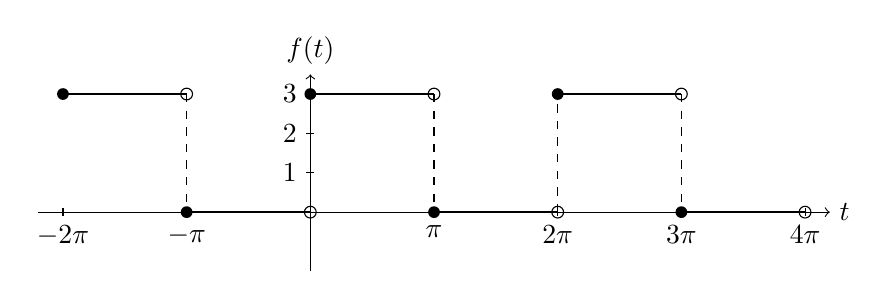
\begin{tikzpicture}[
        scale=0.5, % Updated scale factor to make the figure fit within margins
        % Define a style for the filled circles at the start of steps
        solid_point/.style={circle,fill,inner sep=1.5pt},
        % Define a style for the open circles at the end of steps
        open_point/.style={circle,draw,inner sep=1.5pt}
    ]

    % Define the period
    \def\period{2*pi} % Period is 2*pi

    % Draw the axes
    % Adjusted x-axis range to be from -2.2*pi to 4.2*pi to show periods from -2pi to 4pi
    \draw[->] (-2.2*pi,0) -- (4.2*pi,0) node[right] {$t$}; % Changed x to t
    % Adjusted y-axis range to accommodate values up to 3
    \draw[->] (0,-1.5) -- (0,3.5) node[above] {$f(t)$}; % Changed f(x) to f(t)

    % Draw the grid lines for integer multiples of pi
    % Iterates from -2 to 4 to cover the new x-axis range
    \foreach \i in {-2,...,4}
    {
        \pgfmathsetmacro{\xcoord}{\i * pi}
        \draw (\xcoord,0.1) -- (\xcoord,-0.1) node[below] {
            $\ifnum\i=0\else\ifnum\i=1\pi\else\ifnum\i=-1-\pi\else\i\pi\fi\fi\fi$ % Removed 0pi label
        };
    }
    % Draw the grid lines for y-values 1, 2, 3
    \foreach \y in {1,2,3}
        \draw (0.1,\y) -- (-0.1,\y) node[left] {$\y$};

    % Define the step function for one period:
    % f(t) = 3 for 0 <= t < pi
    % f(t) = 0 for pi <= t < 2pi (period is 2pi)

    % Loop to draw multiple periods
    % Changed loop range to draw periods from -2pi to 4pi
    \foreach \k in {-1,0,1} % Draws periods: [-2pi, 0), [0, 2pi), [2pi, 4pi)
    {
        \pgfmathsetmacro{\offset}{\k * \period}

        % First step: value 3 (from offset to offset + pi)
        \draw[thick] (\offset, 3) -- (\offset + pi, 3);
        \node[solid_point] at (\offset, 3) {};
        \node[open_point] at (\offset + pi, 3) {};

        % Second step: value 0 (from offset + pi to offset + 2*pi)
        \draw[thick] (\offset + pi, 0) -- (\offset + \period, 0);
        \node[solid_point] at (\offset + pi, 0) {};
        \node[open_point] at (\offset + \period, 0) {};

        % Add vertical lines to connect steps
        % This connects the open point of the first step (y=3) to the solid point of the second step (y=0)
        \draw[dashed] (\offset + pi, 3) -- (\offset + pi, 0);

        % Connects the open point of the current period's second step (y=0) to the solid point of the next period's first step (y=3)
        % Only draw for the connections between the displayed periods
        \ifnum\k<1 % Adjusted condition to draw lines for k=-1 and k=0
            \draw[dashed] (\offset + \period, 0) -- (\offset + \period, 3);
        \fi
    }

    \end{tikzpicture}
    \caption{A periodic step function} % Added a caption for the figure
    \label{fig:periodic_step_function} % Added a label for cross-referencing
\end{figure}

\subsection*{The First Term: $a_0$}

First let us differentiate the infinite Fourier Series from $0$ to $2\pi$:

\begin{align}
    \int_0^{2\pi} f(t) \mathrm{d}t & = \int_0^{2\pi} (a_0 + a_1\cos(t) + a_2\cos(2t) + \dots + a_n\cos(nt) + b_1\sin(t) + b_2\sin(2t) + \dots + b_n\sin(nt))\mathrm{d}t\\
    &\text{Using the integrated sine \& cosine identities above:}\\
    & = \int_0^{2\pi} a_0 \mathrm{d}t + \cancel{\int_0^{2\pi} a_1\cos(t) \mathrm{d}t} + \cancel{\int_0^{2\pi} a_2\cos(2t) \mathrm{d}t} + \dots + \cancel{\int_0^{2\pi} a_n\cos(nt) \mathrm{d}t} + \cancel{\int_0^{2\pi} b_1\sin(t) \mathrm{d}t} + \cancel{\int_0^{2\pi} b_2\sin(2t) \mathrm{d}t} + \dots + \cancel{\int_0^{2\pi} b_n\sin(nt) \mathrm{d}t} \\
    & = a_0 \cdot t \bigg\vert_0^{2\pi} \\
    \int_0^{2\pi} f(t) & = a_0 \cdot 2\pi \\
    & \text{Solving for $a_0$:}\\
    a_0 & = \frac{1}{2\pi}\int_0^{2\pi} f(t) \mathrm{d}t
\end{align} 

In other words, $a_0$ is equal to the \textit{mean} of $f(t)$ for the integration period. This makes sense because sine and cosine functions oscillate between $-1$ and $1$, and $a_0$ represents the center starting point for a Fourier Series representation of a periodic function.

\subsection*{The $n$th Coefficients: $a_n$ \& $b_n$}

Now we will solve for the cosine coefficients ($a_n \text{ for } n \in 1, 2, \dots$). First, we multiply our Fourier Series by $\cos(nt)$:

\begin{align}
    f(t)\cos(nt) & = a_0 \cdot \cos(nt) \\& + a_1\cos(t) \cdot \cos(nt) \\& + a_2\cos(2t) \cdot \cos(nt) \\& + \dots \\& + a_n\cos(nt) \cdot \cos(nt) \\& + b_1\sin(t) \cdot \cos(nt) \\& + b_2\sin(2t) \cdot \cos(nt) \\& + \dots \\& + b_n\sin(nt) \cdot \cos(nt)\\
    &\text{Now we can integrate both sides from $0$ to $2\pi$ and eliminate most terms using the trigonometric identies we built above}\\
    \int_0^{2\pi}f(t)\cos(nt)\mathrm{d}t & = \cancel{a_0 \int_0^{2\pi} \cos(nt) \mathrm{d}t} \\& + \cancel{a_1\int_0^{2\pi}(\cos(t) \cdot \cos(nt)) \mathrm{d}t} \\& + \cancel{a_2\int_0^{2\pi}(\cos(2t) \cdot \cos(nt)) \mathrm{d}t} \\& + \dots \\& + a_n\int_0^{2\pi} \cos^2(nt) \mathrm{d}t \\& + \dots \\& + \cancel{b_1\int_0^{2\pi}(\sin(t) \cdot \cos(nt)) \mathrm{d}t} \\& + \cancel{b_2\int_0^{2\pi}(\sin(2t) \cdot \cos(nt)) \mathrm{d}t} \\& + \dots \\& + \cancel{b_n\int_0^{2\pi}(\sin(nt) \cdot \cos(nt)) \mathrm{d}t}\\
    & = a_n \cdot \pi \\
    a_n & = \frac1\pi \int_0^{2\pi} f(t) \cdot \cos(nt) \mathrm{d}t
\end{align}

Similarly, we can solve for the sine coefficients of the infinite Fourier series ($b_n \text{ for } n \in 1, 2, \dots$) by multiplying each side of the series by $\sin(nt)$:

\begin{align}
    f(t)\sin(nt) & = a_0 \cdot \sin(nt) \\& + a_1\cos(t) \cdot \sin(nt) \\& + a_2\cos(2t) \cdot \sin(nt) \\& + \dots \\& + a_n\cos(nt) \cdot \sin(nt) \\& + \dots \\& + b_1\sin(t) \cdot \sin(nt) \\& + b_2\sin(2t) \cdot \sin(nt) \\& + \dots \\& + b_n\sin(nt) \cdot \sin(nt) \\& + \dots \\
    &\text{Now we can integrate both sides from $0$ to $2\pi$ and eliminate most terms using the trigonometric identies we built above}\\
    \int_0^{2\pi}f(t)\sin(nt)\mathrm{d}t & = \cancel{a_0 \int_0^{2\pi} \sin(nt) \mathrm{d}t} \\& + \cancel{a_1\int_0^{2\pi}(\cos(t) \cdot \sin(nt)) \mathrm{d}t} \\& + \cancel{a_2\int_0^{2\pi}(\cos(2t) \cdot \sin(nt)) \mathrm{d}t} \\& + \dots \\& + \cancel{a_n\int_0^{2\pi} \cos(nt) \cdot \sin(nt) \mathrm{d}t} \\& + \dots \\& + \cancel{b_1\int_0^{2\pi}(\sin(t) \cdot \sin(nt)) \mathrm{d}t} \\& + \cancel{b_2\int_0^{2\pi}(\sin(2t) \cdot \sin(nt)) \mathrm{d}t} \\& + \dots \\& + b_n\int_0^{2\pi}\sin^2(nt) \mathrm{d}t \\& + \dots
    & = b_n \cdot \pi \\
    b_n & = \frac1\pi \int_0^{2\pi}f(t) \cdot \sin(nt) \mathrm{d}t
\end{align}

\end{document}
